\documentclass[12pt]{exam}
\usepackage[utf8]{inputenc}
\usepackage{amsmath,amstext,amsthm,amssymb,amsxtra, graphicx}
\usepackage[top=1.5in, bottom=1.5in, left=1.25in, right=1.25in]	{geometry}
%\usepackage[normalem]{ulem}
\usepackage{txfonts} % pxfonts txfonts 
\usepackage[T1]{fontenc}
\usepackage{lmodern}
\renewcommand*\familydefault{\sfdefault}
 \usepackage{euler}   % better than the option below
\usepackage{pdfsync}
\usepackage{multicol}
\newcommand{\ci}[1]{_{ {}_{\scriptstyle #1}}}
\graphicspath{ {images/} }


\newcommand{\norm}[1]{\ensuremath{\left\|#1\right\|}}
\newcommand{\abs}[1]{\ensuremath{\left\vert#1\right\vert}}
\newcommand{\ip}[2]{\ensuremath{\left\langle#1,#2\right\rangle}}
\newcommand{\p}{\ensuremath{\partial}}
\newcommand{\pr}{\mathcal{P}}

\newcommand{\pbar}{\ensuremath{\bar{\partial}}}
\newcommand{\db}{\overline\partial}
\newcommand{\D}{\mathbb{D}}
\newcommand{\B}{\mathbb{B}}
\newcommand{\Sp}{\mathbb{S}}
\newcommand{\T}{\mathbb{T}}
\newcommand{\R}{\mathbb{R}}
\newcommand{\Z}{\mathbb{Z}}
\newcommand{\C}{\mathbb{C}}
\newcommand{\N}{\mathbb{N}}
\newcommand{\Q}{\mathbb{Q}}
\newcommand{\mQ}{\mathcal{Q}}
\newcommand{\mS}{\mathcal{S}}
\newcommand{\scrH}{\mathcal{H}}
\newcommand{\scrL}{\mathcal{L}}
\newcommand{\td}{\widetilde\Delta}
\newcommand{\pw}{\text{PW}}
\newcommand{\esup}{\text{ess.sup}}
\newcommand{\Tn}{\mathcal{T}_n}
\newcommand{\Bn}{\mathbb{B}_n}
\newcommand{\rt}{\mathcal{O}}
\newcommand{\avg}[1]{\langle #1 \rangle}
\newcommand{\one}{\mathbbm{1}}
\newcommand{\eps}{\varepsilon}
\newcommand{\grad}{\nabla}

\newcommand{\La}{\langle }
\newcommand{\Ra}{\rangle }
\newcommand{\rk}{\operatorname{rk}}
\newcommand{\card}{\operatorname{card}}
\newcommand{\ran}{\operatorname{Ran}}
\newcommand{\osc}{\operatorname{OSC}}
\newcommand{\im}{\operatorname{Im}}
\newcommand{\re}{\operatorname{Re}}
\newcommand{\tr}{\operatorname{tr}}
\newcommand{\vf}{\varphi}
\newcommand{\f}[2]{\ensuremath{\frac{#1}{#2}}}

\newcommand{\kzp}{k_z^{(p,\alpha)}}
\newcommand{\klp}{k_{\lambda_i}^{(p,\alpha)}}
\newcommand{\TTp}{\mathcal{T}_p}
\newcommand{\m}[1]{\mathcal{#1}}
\newcommand{\md}{\mathcal{D}}
\newcommand{\qan}{\abs{Q}^{\alpha/n}}
\newcommand{\sbump}[2]{[[ #1,#2 ]]}
\newcommand{\mbump}[2]{\lceil #1,#2 \rceil}
\newcommand{\cbump}[2]{\lfloor #1,#2 \rfloor}

\newcommand{\hn}{{2}}
\newcommand{\dd}{{09-21}}
\newcommand{\class}{Aero 417}
\newcommand{\term}{Fall 2024}
\newcommand{\examnum}{Homework \hn: Due \dd}
\newcommand{\examdate}{}
\newcommand{\timelimit}{75 Minutes}
\newcommand{\vc}[3]{\langle #1,#2,#3\rangle}
\newcommand*{\vv}[1]{\vec{\mkern0mu#1}}
\newcommand{\bv}[1]{\boldsymbol{#1}}
\newcommand{\hide}[1]{}
\newcommand{\uvec}[1]{\boldsymbol{\hat{\textbf{#1}}}}
\newcommand{\vex}[1]{\boldsymbol{{\textbf{#1}}}}
\newcommand{\px}{\frac{\partial}{\partial x}}
\newcommand{\py}{\frac{\partial}{\partial y}}
\newcommand{\pt}{\frac{\partial}{\partial t}}
\newcommand{\pxx}{\frac{\partial^2}{\partial x^2}}
\newcommand{\pyy}{\frac{\partial^2}{\partial y^2}}
\newcommand{\ptt}{\frac{\partial^2}{\partial t^2}}


\pagestyle{head}
\firstpageheader{}{}{}
\runningheader{\class}{ Page \thepage\ of \numpages}{\examnum}
\runningheadrule

\makeatletter
\renewcommand*\env@matrix[1][*\c@MaxMatrixCols c]{%
  \hskip -\arraycolsep
  \let\@ifnextchar\new@ifnextchar
  \array{#1}}
\makeatother

\printanswers
\begin{document}

\noindent
\begin{tabular*}{\textwidth}{l @{\extracolsep{\fill}} r @{\extracolsep{6pt}} l}
\textbf{\class} & \textbf{Name:} & \makebox[2in]{\bf{Benjamin Tollison}}\\
\end{tabular*}\\
\rule[2ex]{\textwidth}{2pt}
%
\begin{questions}
\begin{question}
A jet engine is traveling through the air with the forward velocity of 300 m/s. 
The exhaust gases leave the nozzle with an exit velocity of 800 m/s with respect to the nozzle. If the mass flow rate through the engine is 10 kg/s, determine the jet engine thrust.
The exit plane static pressure is 80 kPa, inlet plane static pressure is 20 kPa, ambient pressure surrounding the engine is 20 kPa, and the exit plane area is 4.0 m$^2$.  
\end{question}
\begin{solutionorbox}[\stretch{1}]
\begin{align*}
\begin{cases}
  V_\infty = 300  \frac{m}{s}\\
  V_e = 800  \frac{m}{s}\\
  P_e = 80  \text{kPa}\\
  P_{\text{atm}} = 20  \text{kPa} \\
  A_e = 4 \, m^2 \\
  \dot{m} = 10  \frac{kg}{s}
\end{cases}
\end{align*}

\[T = \dot{m} V_e - \dot{m} V_\infty + A_e (P_e - P_{\text{atm}})\]
\[\therefore T = 245 \text{kN}\]

\end{solutionorbox}

\newpage 
\begin{question}
Describe the differences between Brayton Cycle and a Real Gas Turbine Cycle. Make
diagrams to explain the losses associated with a real engine.
\end{question}
\begin{solutionorbox}[\stretch{1}]
\[\]
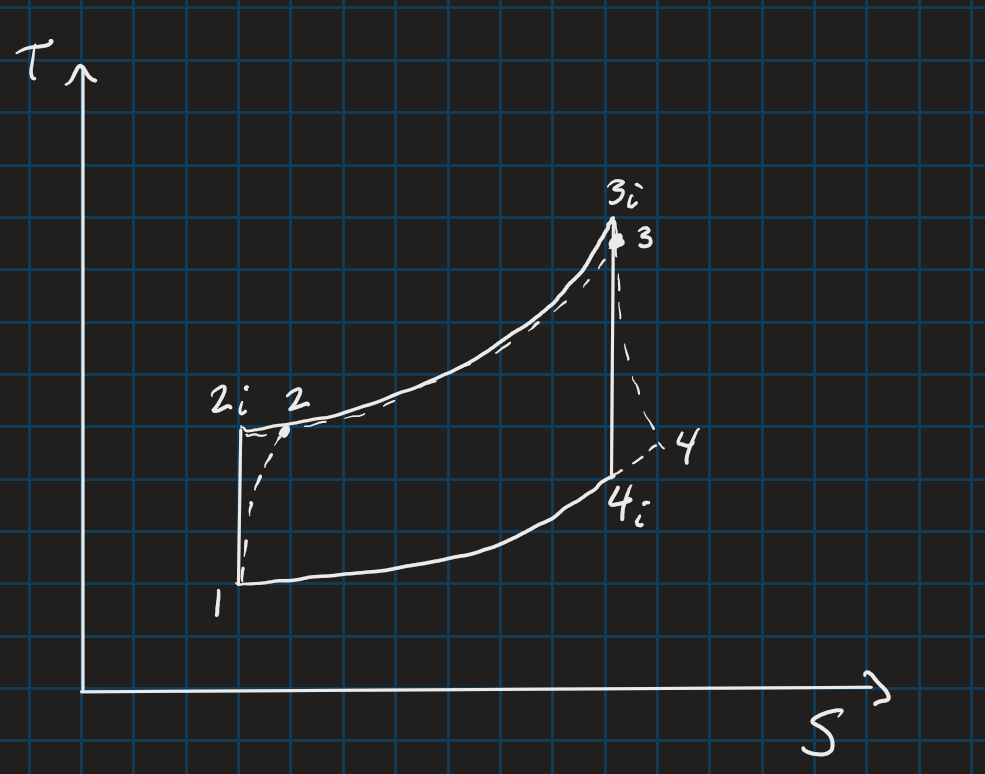
\includegraphics[width=\linewidth]{brayton v real cycle.png}
The first losses occur in the compressor from stage 1->2 due to the 
flow not being reversible. The combustion process is not completely isobaric.
The process in the turbine is also not reversible.
\end{solutionorbox}


\newpage 
\begin{question}
Find all eigenvalues and eigenfunctions for the equation: 
$\varphi'' + \lambda \varphi = 0$ with $\varphi(0) = 0$ and $\varphi'(\pi) = 0.$
\end{question}
\begin{solutionorbox}[\stretch{1}]
\end{solutionorbox}


\newpage 
\begin{question}
Solve 
\begin{align*}
\begin{cases}
\ptt u = \pxx u\\ 
u(0, t) = u(\pi, t) = 0\\ 
u(x,0) = f(x), \pt u(x,0) = 0,
\end{cases}
\end{align*}
where $f(x)$ is the ``hat function'': it's $0$ and $0$ and $\pi$ and $1$ and $\pi/2$ and 
linear in between. 
\end{question}
\begin{solutionorbox}[\stretch{1}]
\end{solutionorbox}


\newpage 
\begin{question}
This is another perspective on the SOV method. Consider the problem 
\begin{align*}
\begin{cases}
\pt u = \pxx u\\
u(0,t) = u(\pi, t) = 0\\ 
u(x,0) = g(x)
\end{cases}.
\end{align*}
For each fixed $x$, assume that the solution can be written as $\sum_{k=1}^{\infty}B_k\sin(kx)$. 
Note that the $B_k$ depend on $t$ so a better way to write it is $\sum_{k=1}^{\infty}
B_k(t) \sin(kx)$. Starting from this point, find the SOV solution. 
(Note: I had a typo that said $B_k(x)$ before; it should be 
$B_k(t)$ SORRY!!)
\end{question}
\begin{solutionorbox}[\stretch{1}]
Plugging the function into the PDE we get: 
\begin{align*}
\sum_{k=1}^{\infty}B_k'(t)\sin kx
&= \sum_{k=1}^{\infty}B_k(t)\frac{d^2}{dx^2}\sin kx
\\&= \sum_{k=1}^{\infty}B_k(t)(-k^2 \sin kx)
\\&= -\sum_{k=1}^{\infty}B_k(t)k^2 \sin kx.
\end{align*}
Subtracting the left from the right: 
\begin{align*}
0 = \sum_{k=1}^{\infty}(B_k'(t) + k^2 B_k(t))\sin kx.
\end{align*}
Since the $\sin kx$ functions are linearly independent, this implies that
for all $k$, $B_k'(t) =- k^2 B_k(t)$. So we get an ODE for $B_k$ and the 
solution is $B_k (t) = B_k(0)e^{-k^2 t}$. To find the values of the 
constants note that: 
\begin{align*}
g(x) 
= u(x,0)
= \sum_{k=1}^{\infty}B_k(0) \sin kx.
\end{align*}
That is, as before, $B_k(0) = \frac{2}{\pi}\int_{0}^{\pi}g(y)\sin ky dy$.
\end{solutionorbox}

\end{questions}
\end{document}
